% {{{ Preamble
\documentclass[a4paper, 11pt, notitlepage]{nsf}
\usepackage{booktabs}
\usepackage{color}
\usepackage{hyperref}
\usepackage{timestamp}
\usepackage{blindtext}
\usepackage{chemarr}
\usepackage{float}
\usepackage{amsmath}
\usepackage{amsfonts}
\usepackage{xspace}
\usepackage{hyperref}
\usepackage{pgfplots}
\usepackage{titling}
\usepackage{mhchem}
%\usepackage{fixltx2e} 
\usepackage{pgfgantt}
\pgfplotsset{compat=1.8}
% \pgfplotsset{every axis/.style={scale only axis}}
% \newcommand{\ug}{$\mathcal{UG}\xspace4$\xspace}
\newcommand{\ug}{uG4\xspace}
\newcommand{\delT}[1]{\frac{\partial #1}{\partial t}}
\newcommand{\ccyt}[0]{c_c}
\newcommand{\cer}[0]{c_e}
\newcommand{\ip}[1]{p}
\newcommand{\cca}[0]{[\mathrm{Ca}^{2+}]}
\newcommand{\cip}[0]{[\mathrm{IP}_3]}
\renewcommand{\abstractname}{Summary}
\renewcommand{\refname}{References}
% }}}

% Authors and Title {{{
\author{Sean Gillian Queisser (PI), Stephan Grein}
\title{Dimension-switching multigrid}
\date{\today}
% }}}

% Begin of document {{{
\begin{document}
% }}}

% Title and Abstract {{{
\maketitle
\begin{abstract}
In this project we intend to develop and test a new dimension-switching multigrid method (DSMG). An important area of future application of this DSMG method is neuroscience, where highly anisotropic computational domains induce very fine 3D coarse grids, making standard geometric multigrid methods inefficient. We plan to study the calcium dynamics in reconstructed neurons, where the endoplasmic reticulum (ER), a multifunctional intracellular organelle of a neuron that consists of a complex three-dimensional network of connected endomembrane tubules, stacks and cisternae, is involved in various ion exchange processes. Of interest here are the three-dimensional spatiotemporal Ca\textsuperscript{2+} and Inositol-3-Phosphate (IP\textsubscript{3}) dynamics in the intracellular space of neurons. We model these biochemical dynamics by a system of diffusion-reaction equations with highly nonlinear flux-boundary conditions and the Poisson-Nernst-Planck (PNP) equations. Using finite volume discretization together with GMG and DSMG, we intend to (1) develop and study our DSMG-related code with respect to scalability and (2) run systematic numerical simulations of the calcium model on a very large, publicly available data set. While only 1d morphological neuron data is directly available, our project requires a detailed 3d representation of the neuronal computational domain. For this we developed an automated pipeline to generate the necessary domains. Thus, we (3) intend to study and reconstruct the \url{www.neuromorpho.org} database using available HPC resources. In total, this project should positively impact the computational mathematics research community, as well as parallel computing and neuroscience fields.
\end{abstract}

% version tag (final)
% \textcolor{green}{\timestamp}
% }}}

% Research Objectives {{{
\section{Research Objectives}
Computational Neuroscience is a rapidly developing research field that demands more and more computing resources for solving complex problems. Where in the past, models of signal processing in brain cells were strongly reduced -- due to the lack of computing power and high resolution experimental data -- they are now being developed in more detail. Emerging areas of research encompass large scale network simulations, three-dimensional simulations of neuronal signals \cite{Xylouris2007, Xylouris2012, Breit2016, Breit2018a, Breit2018b} and multiscale modeling and simulation in neuroscience \cite{Stepniewski2019b}.

In order to resolve biochemical and electrical signals of neurons and networks based on physical first principles, models defined by sets of highly nonlinear and coupled partial and ordinary differential equations need to be numerically and efficiently solved. Models based on partial differential equations (PDEs) furthermore need to be coupled to microscale processes, such as the molecular dynamics of post-synaptic receptors. Thus, solvers for numerical PDEs and molecular dynamics need to be coupled in a multiscale modeling and simulation approach. Resolving ion dynamics at high intracellular resolution is, even with ample computing resources, challenging. In order to cope with the computational complexity of these problems, hybrid dimensional methods need to be developed, where e.g. \emph{high interest} zones are resolved in full three dimensions, whereas \emph{low interest} zones are resolved in two or one dimensions.

The main project below covers the areas of highly detailed three-dimensional modeling and simulation of neuronal processes, multiscale modeling as well as the development of numerical methods for efficiently solving the arising numerical problems on highly parallel computing platforms. The intention within this project is to develop novel numerical strategies and to compute large sweeps of neuroscientific simulation data, in order to support and advance active projects in Computational Neuroscience.

For the proposed sub-projects, the authors have established models, numerical methods and tools in the area of detailed 3d simulations of neuronal processes and multiscale modeling. Having developed the tool \emph{NeuRA} for automated reconstruction of the three-dimensional morphologies of neurons and organelles, \cite{Jungblut2011}, and implemented in CUDA for parallel GPU image reconstruction, the detailed morphology of neuronal architectures and organelles can efficiently be incorporated as a parameter for studies with respect to the morphological influence on signal processing in neurons. Numerical simulations, e.g. of the calcium dynamics within nuclei of hippocampal neurons  \cite{Queisser2008, Wittmann2009}, or the vesicular dynamics in boutons of the \emph{Drosophila} Neuromuscular Junction \cite{Knodel2014}, revealed that the three-dimensional organization of the cellular and intracellular domain can significantly influence the functional implications of biochemical cellular signals. 
With the launch of a project between the groups of Andreas Herz (LMU M\"unchen), Gillian Queisser (Goethe University Frankfurt) and Mark Ellisman (UCSD, San Diego, USA) to decipher the dynamical microscale structure-function relation of dendritic spines, a hybrid 1d/3d model of the Poisson-Nernst-Planck equation was implemented in the simulation environment \ug \cite{Vogel2013, Heppner13}. It is intended to identify the functional consequences of the fine-scale organization of dendritic spines on the macroscopic and system level. The complexity of the underlying numerical problem requires high performance computing in order to solve even reduced test cases. 
These aspects are being further investigated in the context of Transcranial Magnetic Stimulation, a clinical technique used to treat neurological diseases, such as schizophrenia, in an NIH-funded project together with Dr. Opitz (Engineering, University of Minnesota, Minneapolis), Dr. Vlachos (Neurophysiology, University of Freiburg, Germany) and Dr. Jedlicka (Computational Neuroscience, University of Giessen, Germany). 
%Preliminary studies of synaptic contacts between nerve cells have revealed, that the positioning of receptors, the position of vesicle release and the size of the synaptic cleft control the structural switch of N-Cadherin trans-cellular connections \cite{Grein2013, Grein2014b}. Building upon this result, a multi-scale model of the synaptic cleft is being developed, including the macroscopic propagation of ions and neurotransmitters (modeled on the continuum scale) and the microscopic molecular dynamics of receptor/neurotransmitter interaction that triggers postsynaptic currents. The full multiscale coupling is achieved by the integration of Molecular Dynamics simulators, such as NAMD, \cite{Humphrey1996, Phillips2005} or MDCore, in the simulation platform \ug, \cite{Heppner13}. Both tools have been shown to carry excellent scaling properties on the BG/Q architecture, \cite{NamdSC12}.
%
%Focussing on the interaction between N-Cadherin and calcium ions, there remains an open question, whether there may be other factors involved in the binding process between the two, rather than the negatively charged Cadherin sidechains and the divalent positive ion. In preliminary studies carried out using the Molecular Dynamics simulator NAMD, \cite{Phillips2005, Humphrey1996}, the authors have investigated the role of dehydration of the binding site as an additional determinant of calcium binding \cite{Grein2014a}.
In addition to the specific neuroscientific applications, there is a vested interest and activity in developing scalable algorithms and methods for efficiently solving numerical problems of the sort mentioned below. This includes robust solvers for highly nonlinear problems such as the Poisson-Nernst-Planck equations or efficient geometry and grid handling. A major aspect of neuroscientific simulation is the underlying computational domain. Nerve cells typically have very anisotropic structures (tree-like shapes), termed dendrites and axons, that elicit complex branching patterns. A numerically robust discrete representation of these morphologies in the form of volume meshes is needed, that can undergo stable grid-refinement within multi-level solvers, such as geometric multigrid methods. The applicants have developed a novel grid refinement strategy, based on the subdivision volume theory, that produces ideal mixed-element volume grid refinements which can handle highly complex biological morphologies. Preliminary tests show this robustness. More extensive studies in application-relevant benchmarks again require ample computing resources.

% }}}

% Computational Methodology {{{
\section{Computational Methology}
\label{sec:Project-Details}
The simulations of spatio-temporal dynamics outlined in Sec. \ref{sec:research_plan} will be carried out with the multiphysics simulation package uG4 \citep{Vogel2013, Heppner13}. This is a decades-old project focussed on solving partial differential equations on unstructured grids. In particular the code has been developed to run very well on highly-parallel compute architectures \citep{Vogel2013, Heppner13}. For this proposal we will be making use of \textbf{Finite Element/Finite Volume} discretization methods for the underlying systems of partial differential equations. The resulting system of linear equations will be solved using \textbf{Geometric Multigrid} (GMG) or \textbf{Algebraic Multigrid} (AMG) methods, \textbf{Krylov methods}, or a combination of the above where a Multigrid method may function as a preconditioner. In the subproject \emph{DSMG} we intend to test a novel GMG approach that makes use of \textbf{dimension-switching during coarse grid correction} in a highly parallelized situation. 
The simulation framework uG4 is publicly available on Github\footnote{See the various repositories in the organization \texttt{UG4} on \url{https://github.com/UG4}}. Newly developed code will be tested locally, on local clusters and eventually on remote highly parallel architectures. Upon peer-reviewed publication all code will be made publicly available through a repository in the existing Github organization.
Produced simulation results are stored in VTK format (1 file per time step). After completion of a simulation run, e.g. parameter sweeps, we will copy data to a local storage facility. Over the period of an average month we expect to accumulate $<$ 1 TiB of VTK data. 

% }}}

% Application Efficiency {{{
\section{Application efficiency}
The SDSC Comet CPU resource is suitable for our research because it allows
capacity computing and a quick turnaround on small to medium-scaled jobs
for shorter runtimes, which makes it ideal for running exploratory simulations 
with new code features. The large shared memory per node (128 GiB) allows us to load 
large computational grids which would not be possible with the smaller shared memory
per node on comparable resources. Additionally, the TACC Stampede2 system would 
allow us to carry out capability computations and would
be our primary resource for testing scalability of our applications and performing 
fine grain simulations for scientific publication. Production simulations for
 our neurobiological motivated research questions will potentially have a long 
runtime, and Stampede2 allows for long simulations of about 48 hours in the normal 
queues and one might request even longer running jobs in the long queue.
Comparing our demands with the XSEDE Resource Selector\footnote{Information was 
retrieved from \url{https://portal.xsede.org/allocations/resource-info}}
which facilitates users to make a well-grounded decision on how to select a 
compute resource, confirmed our pre-selected resources. Application efficiency 
is documented in the attached file \textit{performance}.

% % Performance and Scaling of ug4 introduction {{{
Our base code \ug is parallelized using MPI and written in C++ and has been extensively 
benchmarked elsewhere (Vogel et al., 2013; Heppner et al., 2013) and shown to scale to $>$ 200,000 processes. The solver interfaces of \ug are designed with parallel computing in mind. The first benchmark or standard test problem is the Laplace equation in three dimensional space on a unit cube. The second order elliptic partial  differential equation reads, where $\Phi$ is a scalar function in the domain $\Omega \subset \mathbf{R}^n$, and $\Delta$ is the Laplace operator:
\begin{equation}
\Delta \Phi = 0
\end{equation}

Strong scaling is demonstrated for a sevenfold regularly refined unit cube, cf.
Tab. \ref{tab:xsede_strong_scaling} and Fig. \ref{fig:speedup_laplace}. The execution time roughly halves by doubling the number of processes. A weak scaling study, cf. Tab. \ref{tab:xsede_weak_scaling} and Fig. \ref{fig:scaled_speedup_laplace}, \ref{fig:scaled_speedup_laplace2} on SDSC Comet and TACC Stampede2  confirms the scaling behavior. With each refinement of the grid the degrees of freedom (DoFs) increase by a factor of 8 and thus we increased the number of processes eightfold in each refinement step.
% }}}

% {{{ 3d Laplace problem
\begin{center}
\begin{table}[H]
\centering
\begin{tabular}{lrrr} 
\toprule
Strong scaling for first problem in \ug \\
\midrule 
\emph{DoFs} & \emph{Runtime [s]} & \emph{\# Processes} & \emph{\# Nodes}\\
\midrule 
16,974,593 & 41 &  24 & 1 \\
16,974,593 & 20 &  48 & 2 \\
16,974,593 & 14 &  72 & 3 \\
16,974,593 & 10 &  96 & 4 \\
16,974,593 &  8 & 120 & 5 \\
16,974,593 &  7 & 144 & 6 \\
16,974,593 &  5 & 168 & 7 \\
16,974,593 &  2 & 192 & 8 \\
\bottomrule
\end{tabular}
\caption{Runtimes of simulations of a \textbf{3d Laplace problem} on a fixed unit
 cube domain (seven regular refinements) with \ug on the SDSC Comet HPC cluster.
Note that each node can allocate at maximum 24 processes and the maximum number
of processes or cores per job is limited to 1728 processes in total.}
\label{tab:xsede_strong_scaling}
\end{table}
\end{center}

\begin{figure}[H]
\centering
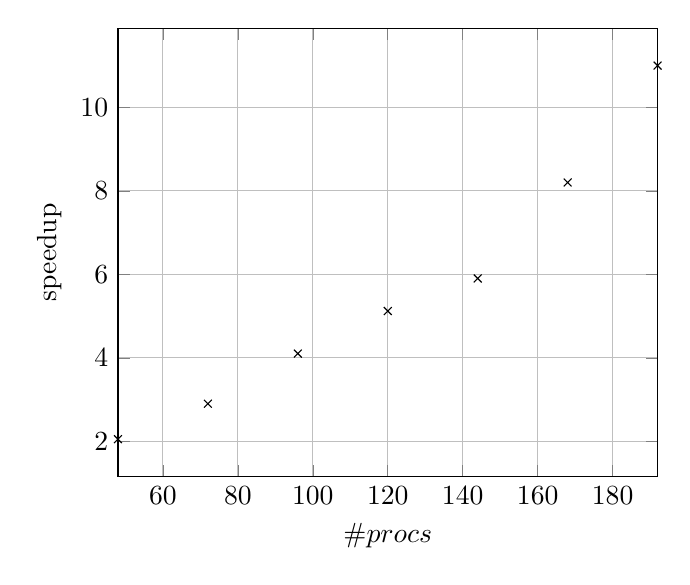
\begin{tikzpicture}
       \begin{axis}[%
            ,xlabel=$\#procs$
            ,ylabel=speedup
            ,grid=major,
            ,xmin=48,
            ,xmax=192]
            \addplot[color=black,only marks, mark=x] coordinates {(48,2.05) (72, 2.9) (96, 4.1) (120, 5.12) (144, 5.9) (168, 8.2) (192, 11)};
        \end{axis}
\end{tikzpicture}
\caption{Speedup of distributed execution. \#procs denotes the involved processes on the SDSC system Comet.}
\label{fig:speedup_laplace}
\end{figure}

\begin{center}
\begin{table}[H]
\centering
\begin{tabular}{lrrr} 
\toprule
Weak scaling for first problem in \ug \\
\midrule 
\emph{DoFs} & \emph{Runtime [s]} & \emph{\# Processes} & \emph{\# Grid refinements} \\
\midrule 
27 & 5.06 & 1 & 0 \\
216 & 5.06 & 8 & 1 \\
1,726 & 6.92 & 64 & 2 \\
13,824 & 6.92 & 512 & 3 \\
110,592 & 5.50 & 4096 & 4 \\
\bottomrule
\end{tabular}
\caption{Runtimes of simulations of a \textbf{3d Laplace problem} on a unit cube 
domain (different number of regular refinements) with \ug on the SDSC Comet HPC cluster.
Note that each grid refinement increases the DoFs by a factor 8.}
\label{tab:xsede_weak_scaling}
\end{table}
\end{center}

\begin{figure}[H]
\centering
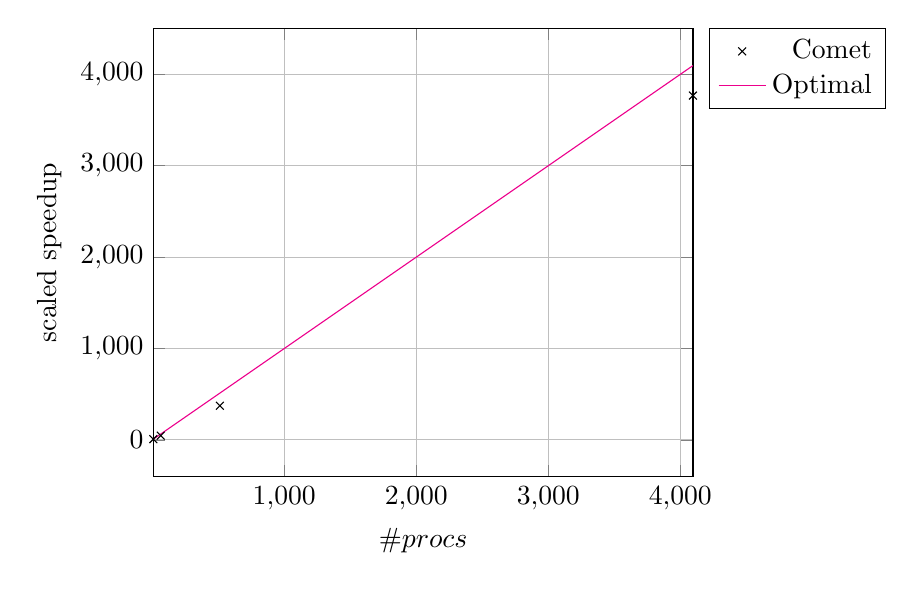
\begin{tikzpicture}
       \begin{axis}[%
            ,xlabel=$\#procs$
            ,ylabel=scaled speedup
            ,legend style={
               cells={anchor=east},
               legend pos=outer north east,
            }
            ,grid=major
            ,xmin=8,
            ,xmax=4096]
            \addplot[color=black,only marks,mark=x] coordinates {(8, 8.0) (64, 46.7) (512, 374.0) (4096, 3768.0) };
            \addplot[color=magenta] coordinates {(1,1) (4096, 4096)};
            \legend{Comet, Optimal}
        \end{axis}
\end{tikzpicture}
\caption{Scaled speedup of distributed execution. \#procs denotes the involved processes on the SDSC system Comet. Note the optimal scaling and achieved scaling behaviour of the test problem.}
\label{fig:scaled_speedup_laplace}
\end{figure}

\begin{center}
\begin{table}
\centering
\begin{tabular}{lrrr} 
\toprule
Weak scaling for first problem in \ug \\
\midrule 
\emph{DoFs} & \emph{Total runtime [s]} & \emph{\# Processes} & \emph{\# Grid refinements} \\
\midrule 
27 & 1 & 1 & 0 \\
216 & 1 & 8 & 1 \\
1,726 & 1 & 64 & 2 \\
13,824 & 1 & 512 & 3 \\
110,592 & 1 & 4096 & 4 \\
884,736 & 2 & 32768 & 5 \\
\bottomrule
\end{tabular}
\caption{Runtimes of simulations of a \textbf{3d Laplace problem} on a unit cube 
domain (different number of regular refinements) with \ug on the TACC Stampede2 HPC cluster.
Note that each grid refinement increases the DoFs by a factor of 8. Note that the \textbf{large} queue
on Stampede2 is not yet available to us to benchmark, thus we are restricted to process count up to 32768.}
\label{fig:xsede_weak_scaling}
\end{table}
\end{center}

\begin{figure}
\centering
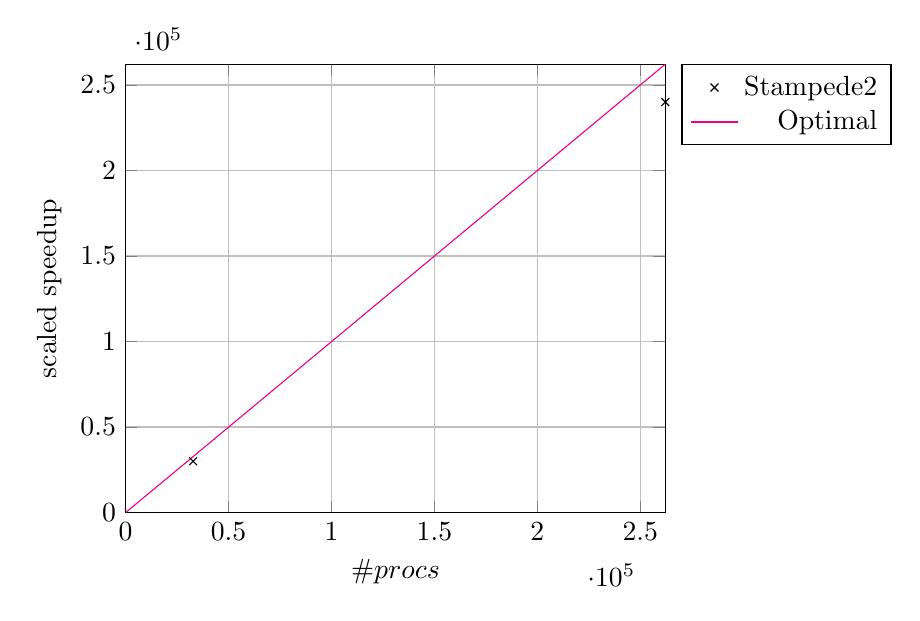
\begin{tikzpicture}
       \begin{axis}[%
            ,xlabel=$\#procs$
            ,ylabel=scaled speedup
            ,legend style={
               cells={anchor=east},
               legend pos=outer north east,
            }
            ,grid=major
            ,xmin=8,
            ,xmax=262144
            ,ymin=1
            ,ymax=262144]
            \addplot[color=black,only marks,mark=x] coordinates { (1,1) (32768, 30000) (262144, 240000)};
            \addplot[color=magenta] coordinates {(1,1) (32768, 32678) (262144, 262144) };
            \legend{Stampede2, Optimal}
        \end{axis}
\end{tikzpicture}
\caption{Scaled speedup of distributed execution. \#procs denotes the involved processes on the TACC system Stampede2. Note the optimal scaling and achieved scaling behaviour of the test problem.}
\label{fig:scaled_speedup_laplace2}
\end{figure}
% }}}

% Spine problem {{{
The second problem is motivated by neurobiology.
Of interest are the three-dimensional spatio-temporal $\textrm{Ca}^{2+}$ and $\textrm{IP}_3$ dynamics in the intracellular space of a neuron respectively spine.
This is modeled by a (system) of diffusion-reaction equations, cf. Eqns. 3-7 
in proposal.
\begin{equation}
\frac{\partial u}{\partial t} = \nabla \cdot (D \nabla u)
\end{equation}
where $u(x, t)$ stands for one of the quantities above.

\noindent The full domain equations for cytosolic calcium and calbindin are thus given by
\begin{align}
  \delT{\ccyt} & \;=\; \nabla \cdot \left( D_{c} \nabla \ccyt \right) \;+\;
    \left(\kappa_{b}^{-}\left(b^{\mathrm{tot}}-b\right)
        -\kappa_{b}^{+}\:b\:\ccyt\right), \label{eq:ccyt}\\
  \delT{b} & \;=\; \nabla \cdot \left( D_{b} \nabla b \right) \;+\;
    \left(\kappa_{b}^{-}\left(b^{\mathrm{tot}}-b\right)
        -\kappa_{b}^{+}\:b\:\ccyt\right)  \label{eq:buff}
\end{align}

 The computational grid is the reconstruction of a synaptic spine in three-dimensional space as depicted in the accompanying proposal document. Starting on the base level with a large number of DoFs the grid is refined three times. The cost for solving the problem increases only slightly but remains bound up to the testable limit, cf. scaling in Fig. \ref{fig:scaled_speedup_spine} and Tab. \ref{tab:spine_speedup}.
% {{{ 3d spine problem 
\begin{center}
\begin{table}[H]
\centering
\begin{tabular}{lrrr} 
\toprule
Weak scaling for second problem in \ug \\
\midrule 
\emph{DoFs} & \emph{Runtime [s]} & \emph{\# Processes} & \emph{\# Grid refinements} \\
\midrule 
547,348 & 37.1 & 24 & 0 \\
4,378,784 & 44 & 192 & 1 \\
35,030,272 & 57 & 1536 & 2 \\
\bottomrule
\end{tabular}
\caption{Runtime of a simulations on a \textbf{spine} reconstruction in three-dimensional
space. Note the grid has been regularly refined two times with \ug and the DoFs 
increase by a factor 8 and thus also the processes have to increase eightfold. Runtime cost
increases slightly but remains bound.}
\label{tab:spine_speedup}
\end{table}
\end{center}

\begin{figure}[H]
\centering
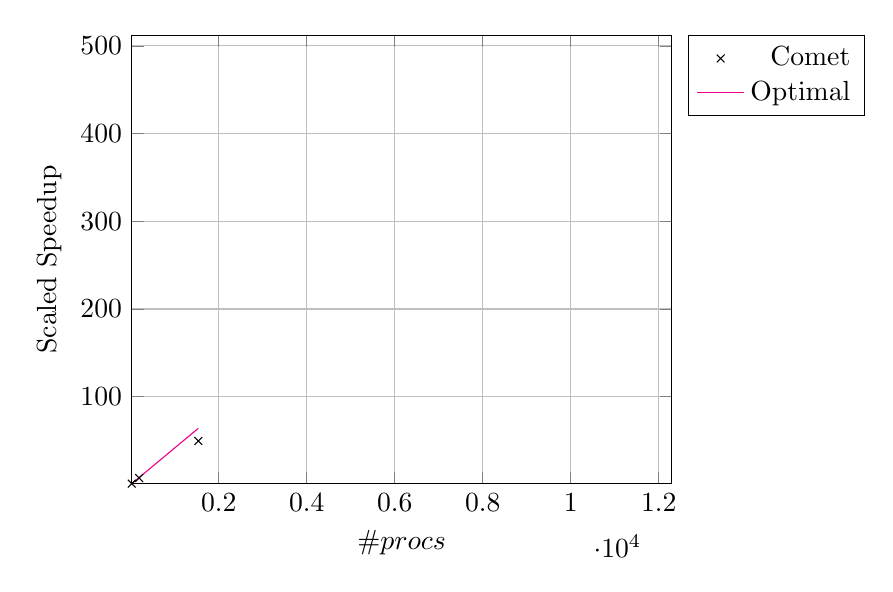
\begin{tikzpicture}
       \begin{axis}[%
            ,xlabel=$\#procs$
            ,ylabel=Scaled Speedup
            ,legend style={
               cells={anchor=east},
               legend pos=outer north east,
            }
            ,grid=major
            ,xmin=24,
            ,xmax=12288
            ,ymin=1
            ,ymax=512]
            \addplot[color=black,only marks,mark=x] coordinates {(24, 1.0) (192, 7.4) (1536, 49.6) };
            \addplot[color=magenta] coordinates {(24, 1.0) (192, 8) (1536, 64)};
            \legend{Comet, Optimal}
        \end{axis}
\end{tikzpicture}
\caption{Scaled speedup of distributed execution. \#procs denotes the involved processes on the SDSC system Comet.}
\label{fig:scaled_speedup_spine}
\end{figure}
% }}}
% }}}

% }}}

% Computational Research Plan {{{
\section{Computational Research Plan}
\label{sec:research_plan}
\paragraph{Poisson-Nernst-Planck (PNP)}\label{subproject:PNP}
In this sub-project, the goal is to develop functionality for the detailed simulation of ionic dynamics in dendritic spines using the Poisson-Nernst-Planck system (``electro-diffusion''):
\begin{align}
  \frac{\partial c_{i}}{\partial t} \:& = \:  \nabla\cdot\left(D_{i}\nabla c_{i}+D_{i}
    \frac{z_{i}F}{RT}c_{i}\nabla\Phi\right) \label{eq:pnp_species}\\
  -\nabla(\varepsilon_{r}\varepsilon_{0}\nabla\Phi) \: & = \:
    \rho_{f}+\sum_{i}z_{i}Fc_{i} \label{eq:pnp_potential}
\end{align}
Equation (\ref{eq:pnp_species}) represents electro-diffusion for various ion species
$c_i$ with $D_i$ being diffusion coefficients; $z_i$ the ions' valencies; $F$, $R$
the Faraday and universal gas constants, respectively, and $T$ the temperature.
Equation (\ref{eq:pnp_potential}) is the Gauss law stating that the charged ions are
the sources for the electric field, represented by the negative gradient of the
electric potential $\Phi$. Here, $\varepsilon_r$, $\varepsilon_0$ are relative
permettivity and vacuum permettivity, resp.; $\rho_f$ is a fixed surface charge density.
\vspace{0.3cm}

The need for simulating ion movement, especially with regard to their
electrical properties, arises from the presence of charged filaments and membranes
throughout the neuron and notably at synapses. The effect of these charges on the
signal transduction and long-term development of neurons remains largely unclear.
Detailed simulations will shed light on the ion dynamics in domains on the micro-
and nano-scale present at, e.g., synaptic spines.

The agglomeration of ions at fixed surface charges is what makes this problem
computationally difficult: As equally charged ions are repelled and oppositely
charged ions are attracted, locally very steep concentration and with that:
very steep potential gradients form at these surfaces and the non-linear term
$c_{i}\nabla\Phi$ in equation (\ref{eq:pnp_species}) becomes very prominent,
making direct coupled solution of the system difficult.
\vspace{0.3cm}

Having run a first set of simulations on artificial dendritic spines with idealized longitudinal filaments inside the neck,
the next step will be to ascertain whether direction-specific effects can be
observed with differently oriented artificial filaments. In particular realistic
reconstructions of single spines and cells became recently
 available to this project which motivates using the realistic cell reconstructions
for simulations which aligns with another project initiated focusing on the
simulation of transcranial magnetic stimulation (TMS). Large-scale simulations
of TMS-induced calcium dynamics in spines and neurons using
the available cell reconstruction are planned. First proof-of-principle simulations
on the reconstruction, are shown in Fig.~\ref{fig:spine_simulation} (see Fig.~\ref{fig:spine} for an example of a spine geometry).

\begin{figure}[h!]
\centering
\includegraphics[scale=0.15]{inc/img/new_spine_simu.png}
\caption{\textbf{Simulation} run of the PNP model on a genuine reconstruction of a spine as displayed
in Fig. \ref{fig:spine}. Simulation time captured 10 ms, snapshots are taken (top left to bottom right) in 2.5 ms intervals.}
\label{fig:spine_simulation}
\end{figure}

\begin{figure}[h!]
\centering
\includegraphics[scale=0.15]{inc/img/spine.png}
\caption{\textbf{Spine geometry}. Depicted is a human spine (yellow) reconstruction with
the common parts dendrite (red), presynapse (magenta), the post synaptic density (cyan)
and the endoplasmic reticulum hidden within the spine.}
\label{fig:spine}
\end{figure}

\noindent \textbf{Estimate of proposed simulation runs:} 48,080, divided into 48,000 runs of shorter 
length on SDSC Comet and and 80 longer runs on TACC Stampede2 for detailed simulations on the TMS project. 
Coarse grain simulation runs on reconstructed spines will be conducted on 10 spines in total.
Parameters to vary: Channel densities (6), boundary conditions (4), initial conditions (4),
each parameter is varied 20 times for parameter sweeps, totaling $10 \times 6 \times 10 \times 4
\times 20 = 48,000$ runs. Towards publication-level simulations, 20 spines will be analyzed with critical parameter sets (4) on high
resolution, thus totaling 80 runs on Stampede2. For a comprehensive overview of the parameter sets we refer to \cite{Breit2018b}.

\paragraph{Dimension-switching multigrid (DSMG)}
In this sub-project the calcium dynamics in a compartmentalized neuron will be modeled.
The endoplasmic reticulum (ER) is a multifunctional intracellular organelle of a neuron,
which consists of a complex three-dimensional network of connected endomembrane
tubules, stacks and cisternae, and is involved in various ion exchange processes,
%cf. Fig.~\ref{fig:schematics},
\cite{Breit2018}, ultimately responsible for synaptic plasticity, `cell within a cell'
structure, cf. \cite{Berridge1998}.

\begin{figure}
\centering
\includegraphics[scale=0.25]{inc/img/schematics.png}
\caption{\textbf{Model geometry}. Simulation domain and model components. The example domain is a cylindrical dendrite 50 $\mu$m in length with variable radius containing a centrally positioned cylindrical ER of variable radius. The rotational symmetry of the domain was used to reduce the problem to two dimensions (axial and radial position). The calcium model contains calcium in the cytosol and the ER as well as calbindin (CalB) in the cytosol. The dynamics of both are governed by a diffusive process and a buffering reaction. Calcium can cross the ER membrane through RyR channels and SERCA pumps, the plasma membrane through PMCA and NCX pumps.}
\label{fig:schematics}
\end{figure}

Of interest are the three-dimensional spatio-temporal $\textrm{Ca}^{2+}$ and $\textrm{IP}_3$ dynamics in the intracellular space of a neuron.
This is modeled by a system of diffusion-reaction equations described in the following.
The boundary conditions for this partial differential equation system are specifed by certain $\textrm{Ca}^{2+}$ and $\textrm{IP}_3$-dependent fluxes which depend on the chosen electrophysiogical stimulation protocol of the neuron.
Mobility in the neuron respectively ER is described by diffusion equations for the four quantities calcium (cytosolic ($c_c$) and endoplasmic ($c_e$)), calbindin-D28k ($b$), and $\textrm{IP}_3$ ($p$), which is required to model $\textrm{IP}_3$ receptors embedded in the endoplasmic membrane
\begin{equation}
\frac{\partial u}{\partial t} = \nabla \cdot (D \nabla u)
\end{equation}
where $u(x, t)$ stands for the four quantities mentioned above.
The diffusion constants $D$ are defined by data available in the literature \cite{Allbritton1992, Schmidt2003}.
The interaction between cytosolic $\textrm{Ca}^{2+}$ calbindin-$\textrm{D}_{28k}$ (CalB) is described by:
\begin{align}
  \mathrm{Ca}^{2+}+\mathrm{CalB}\;\xrightleftharpoons
  [\kappa_{b}^{-}]{\kappa_{b}^{+}}\;[\mathrm{CalBCa}^{2+}].
\end{align}

\noindent The full domain equations for cytosolic calcium and calbindin are thus given by
\begin{align}
  \delT{\ccyt} & \;=\; \nabla \cdot \left( D_{c} \nabla \ccyt \right) \;+\;
    \left(\kappa_{b}^{-}\left(b^{\mathrm{tot}}-b\right)
        -\kappa_{b}^{+}\:b\:\ccyt\right), \label{eq:ccyt}\\
  \delT{b} & \;=\; \nabla \cdot \left( D_{b} \nabla b \right) \;+\;
    \left(\kappa_{b}^{-}\left(b^{\mathrm{tot}}-b\right)
        -\kappa_{b}^{+}\:b\:\ccyt\right)  \label{eq:buff}
\end{align}

\noindent Exponential IP\textsubscript{3} decay towards a basal IP\textsubscript{3} concentration
$p^r$ in the cytosolic space is modeled by a reaction term that is added to the
IP\textsubscript{3} diffusion equation, leading to the diffusion-reaction equation
\begin{align}
  \delT{\ip3} & \;=\; D_p\Delta\ip3 \;-\; \kappa_{\ip3}\left(\ip3-{\ip3}^{r}\right)
\end{align}
for IP\textsubscript{3} in the cytosolic domain.
Endoplasmic Ca\textsuperscript{2+} dynamics are modeled by simple diffusion
\begin{align}
  \delT{\cer} & \;=\; D_{c}\Delta\cer
\end{align}
in the endoplasmic domain. For numerical simulations, the four equations are
discretized in space using a finite volumes method, \cite{Eymard2000}.
%Control volumes are constructed as a Voronoi-like dual tesselation of the original
%tetrahedral mesh by connecting the mid-points of edges, faces and volumes through planar facets.
%The equations above must hold for all control volumes, giving rise to one equation per control volume.
Time discretization is realized using a backwards Euler scheme. The described PDE problem
should be solved by a multigrid method, \cite{Brandt1977,Fedorenko1962,Hackbusch1976,Ruge1987}.
 If one designates with $\Omega_1$ the coarse domain and with $\Omega_2$ the fine
 domain and we require that the domains are nested, i. e. $\Omega_1 \subset \Omega_2$, and a restriction
operator $\mathcal{R}$ and a prolongation operator $\mathcal{P}$ exist one
can write the two grid iteration matrix by
\begin{equation}
u^{(i+1)} = G_2^{\nu_2}(Id - \mathcal{P}A_1^{-1}\mathcal{R}A_2)G_1^{\nu_1} u^{(i)} + \mathcal{P} A_1^{-1}\mathcal{R}f_2,
\end{equation}
where $Id$ is the identity matrix, $G_2$ a post smoothing matrix applied $\nu_2$ times, $G_1$ a pre smoothing matrix
applied $\nu_1$ times, $A_1$ and $A_2$ the matrices arising from the discretized PDE problem on the coarse respectively
fine domains $\Omega_1$ and $\Omega_2$ and $f_2$ the corresponding right hand side of the equation system arising by
discretization on the coarse domain $A_2 u_2 = f_2$. 

In traditional multigrid methods the restriction and prolongation operators are defined
between the same space dimension, i.e. information transfer from a coarse to a fine
grid level within the multigrid hierarchy. The \textbf{dimension-switching multigrid approach} 
we are developing will involve a new multigrid base level of reduced dimensionality, 
which will decrease computational cost. Some of the open topics are convergence rates and parallelization strategies.


\noindent \textbf{Estimate of proposed simulation runs:} 150 runs.
Approximately 50 shorter runs for development of the (parallel) correctness of the MPI program and to improve the parallel efficiency 
of the novel DSMG method and to demonstrate the scaling behaviour of the method will be required. 
Additionally the numerics of the newly developed DSMG algorithm needs to be compared to a standard
numerical problem, a time-dependent convection-diffusion equation on a reconstructed
neuron. To test for robustness of the numerical code 10 cells will be reconstructed,
5 simulation setups (boundary conditions and initial conditions will be varied around a reference case) 
will be run with the standard multigrid algorithm and 5 simulation setups will be run with the new
DSMG algorithm. Results of the runs each will be compared concerning convergence and precision
of the simulation result and contrasted with the results published in \cite{Breit2018}.

\paragraph{Network simulations of electrical and calcium dynamics (NET/CD)}
We have been been developing simulation techniques
for large-scale neuronal network simulations of networks described by graphs  (``1d'') with a
diameter information attached to the vertices (representing idealized, cylindrical or
cone-frustum compartments). The main results from this have been published in \cite{Breit2016}.
We have also developed functionality to couple these large-scale 1d network simulations to fully
resolved 3d reconstructed single-cell calcium simulations (similar to what is described in
\cite{Grein14}). In this kind of simulation, we aim to understand the functional role of calcium
as a messenger, taking into account the endoplasmic reticulum (ER) and a detailed model of the
calcium dynamics including buffers as well as important endoplasmic and plasma membrane calcium
exchange mechanisms such as the IP\textsubscript{3}R and RyR channels, voltage-dependent calcium
channels, and sarco-/endoplasmic reticulum or plasma membrane calcium ATP-ases \cite{Breit13, Breit2018a, Breit2018b}.
As the calcium dynamics are of special interest in the context of synaptic activity (e.g.,
synapse-to-nucleus communication), examining a single fully resolved cell within an active
network allows us to provide realistic synaptical inputs for the calcium simulation.
But even with rather artificial inputs (as, e.g., given by an experimental stimulation protocol),
single-cell calcium simulations and high-detail simulations of small regions of interest (as the
vicinity of one or more dendritic spines) have become more and more important in our ongoing work.

We would like to bring many aspects of the previous work together:
The goal is to investigate whole-cell calcium dynamics on the basis of realistic synaptic input
and membrane potential data from the 1d network model. In view of our basic parameter study
about the influence of geometric parameters on calcium wave elicitation, we want to assess
whether and under which circumstances calcium waves can occur within neurons in an active network:
Which synaptic input patterns can lead to such waves? Can a single firing synapse cause a calcium
signal cascade to the soma? Is the position of the synapse important (because of the
location-specific geometry of the dendrites and ER)? Or are action potentials the only way to
cause calcium influx into the soma (via voltage-dependent calcium channels)?
What is the role of back-propagating action potentials? Do they significantly affect the local
(synaptic) or even global calcium levels?
Investigating these kinds of questions in simulations has been a long-standing goal of our
research with implications for learning and cell survival. In past efforts a grid generation pipeline was developed with the
goal in mind to reconstruct arbitrary cells from the \textit{Neuromorpho.org} database \cite{Ascoli2007}
for the DMSG project and create a multigrid hiearchy. Existing tools, cf. \cite{Moerschel2017}, generated base levels too
fine grained and thus not suitable for HPC solvers. A new ansatz was made by
using spline data and grid generation tools from \ug which use point-diameter data.
Volume meshes are generated efficiently by grid generation algorithms for constrained
Delaunay triangulation \cite{Shewchuk2002, Si2005}. Based on these recent advances
this sub-project aims to investigate by systematic parameter studies the calcium
dynamics using the PNP model in the reconstructed cells on the sub-cellular level.

\noindent \textbf{Estimate of proposed simulation runs:} 1010 runs.
During development some performance bottlenecks where introduced by design of simplicity in the 1d/3d coupling method.
For optimization and increasing the fraction of parallel code and thus to improve scaling
approximately 10 runs will be needed to vary parts of the algorithm for benchmarking
and optimization. An average neuron in the Neocortex has roughly 1000 synapses,
 cf. \cite{Drachman2004}. 1000 runs (Synapse location will be varied)
for production will be used to assess if a \textit{single} firing synapse can cause a signal cascade up to the soma. 

\begin{figure}[!h]
\centering
\includegraphics[scale=0.20]{inc/img/mesh.png}
\caption{\textbf{Grid hierarchy} which shows a neuron with ER on the base level
 (wireframe mesh) and the new coarse level (1d line segments).}
\label{fig:base_level}
\end{figure}

Resources will be used for testing new methods and for running production code. All participants in the project will have access to a shared file in which an estimated demand for compute time for the following project month can be submitted. Stephan Grein will coordinate the internal distribution of compute time for the subsequent month by weighing the individual demand against mile stone deadlines, demand for conference contributions, theses finalizations and other constraint parameters. Through this method, contingent overflow as well as monthly over-demand can be minimized. A preliminary year schedule is provided below in the Ganttchart.

\begin{ganttchart}[vgrid, hgrid, bar/.style={fill=blue!50},
                    y unit chart = 0.4cm, y unit title = 0.4cm, title height=1,
                    bar height=0.4]{1}{12}
  \scriptsize
  \gantttitle{Project Month}{12} \\
  \gantttitlelist{1,...,12}{1} \\
  \ganttgroup{\textbf{PNP}}{1}{12} \\
    \ganttbar[bar/.style={fill=red}]{\scriptsize electro-diffusion through reconstructed patches}{1}{6}\\
    \ganttbar[bar/.style={fill=red}]{\scriptsize TMS simulations on reconstructed spines}{7}{12} \\
  \ganttgroup{\textbf{DMSG}}{1}{12} \\
    \ganttbar[bar/.style={fill=red}]{\scriptsize develop grid generation methods}{1}{3}\\
    \ganttbar[bar/.style={fill=red}]{\scriptsize develop dimension-switching multigrid (MG) methods}{4}{9}\\
    \ganttbar[bar/.style={fill=red}]{\scriptsize bechmark dimension-switching MG and conduct parameter study}{9}{12} \\
  \ganttgroup{\textbf{NET/CD}}{1}{12} \\
    \ganttbar[bar/.style={fill=red}]{\scriptsize large-scale whole-cell simulations}{1}{9} \\
    \ganttbar[bar/.style={fill=red}]{\scriptsize calcium waves in coupled network/whole-cell simulations}{1}{8} \\
    \ganttbar[bar/.style={fill=red}]{\scriptsize back-propagating APs in 1d/3d coupled simulations}{10}{12} \\
    \ganttbar[bar/.style={fill=red}]{\scriptsize systematic TMS simulations on networks/whole-cell}{10}{12} 
\end{ganttchart}

Numerical experiments will be designed by the PI and Stephan Grein, setup, submissions 
to the cluster and data analyis of the results is conducted by Stephan Grein.

\paragraph{PNP}
Examine the electro-diffusion properties through reconstructed pathes of actin and filament networks. 
Examine TMS simulations on detailed anatomical reconstructions of dendritic spines.

\paragraph{DSGM}
Develop and benchmark grid generation with refinement projectors, develop the dimension-switching multigrid operators and benchmark and conduct parameter study of the surrogate
neurobiological problem.

\paragraph{NET/CD}
Large-scale whole-cell simulations of \textit{Neuromorpho.org} \cite{Ascoli2007} database.
Investigating calcium waves in coupled network/whole-cell simulations, back-propagating
action potentials in 1d/3d coupled simulations and systematic TMS simulations on networks/whole-cell

% }}}

% Justification of Resources Requested {{{
\section{Justification of Resources Requested}
The charge unit for SDSC Comet is the Service Unit (SU). One SU corresponds to the use of one compute
core for one hour, accordingly the requested SUs for the sub-projects in this proposal are summarized
in Tab. \ref{tab:sus} below, which are calculated as: $$SUs = \sum Runtime~[h]\quad \times\quad \#~Cores$$
Since the charge unit for TACC Stampede2 varies between the value of 0.8 SU (KNL queue) and 1.0 SU (SKX queue) we estimate the runtimes on Stampede2 with the greater value to be on the safe side.

\begin{table}
\resizebox{\columnwidth}{!}{%
\tiny
\begin{tabular}{llrrrrr}
   \hline\hline
   \multicolumn{7}{l}{Compute time requirements for \textbf{SDSC Comet}}\\
   \hline
   Sub-project &  Type     & \# runs   & \# steps/ & Wall time/    & \# cores/ & Total \\
            &  of run      &           &  run      &  step [hours] &  run      &  [core-h] (SU) \\
   \hline\hline
   PNP      & production  &   19200    &    10     &   0.01         &  1,200    &  2,304,000 \\
   \hline
   DMSG     & development  &    50     &    10      &     0.3       &  2,000   &   300,000 \\
            & production   &   100     &    10      &     0.1       & 3,200   &   320,000 \\
   \hline
   NET/CD   & development  &    10     &    10     &   0.1         &  1,200    &     9,600 \\
            & production   &  1000     &    10     &   0.01        &  2,400    &   240,000 \\
   \hline
   TOTAL    &              &           &           &               &           &  3,053,600 \\
   \hline\hline
\end{tabular}}
\caption{Total number of SUs on SDSC Comet for the sub-projects requested}
\label{tab:sus}
\end{table}

\begin{table}
\resizebox{\columnwidth}{!}{%
\tiny
\begin{tabular}{llrrrrr}
   \hline\hline
   \multicolumn{7}{l}{Compute time requirements for \textbf{TACC Stampede2}}\\
   \hline
   Sub-project &  Type     & \# runs   & \# steps/ & Wall time/    & \# cores/ & Total \\
            &  of run      &           &  run      &  step [hours] &  run      &  [core-h] (SU) \\
   \hline\hline
   PNP      & production   &    20     &    10     &   0.05        &  64,000    &  640,000 \\
   \hline\hline
   DSMG 
            & production   &    10     &    10     &   0.1        &  64,000    &   640,000  \\
    
   \hline
   TOTAL    &              &           &           &               &           &   1,280,000 \\
   \hline\hline
\end{tabular}}
\caption{Total number of SUs on TACC Stampede2 for the sub-projects requested}
\label{tab:sus2}
\end{table}

During simulations data will be stored in the common VTK format. Since dealing with
reconstructions of spines and a large database sweep of to-be-reconstructed cells
additional mid-term storage on Data Oasis of approximately 700 GiB will be requested.
The amount stems from the following calculation: The average grid size of our model
domain is in the range of about 10-100 MiB and one deals with time-dependent problems,
thus, each timestep will save a snapshot of the simulation. Carrying out multiple
runs for production, e.g. 40, cf. Tab. \ref{tab:sus} PNP problem third column.
and 25 timesteps will already use roughly 100 GiB of data. For DSMG problems grids 
need to be refined but less timesteps are carried out typically, still the degree of
freedoms of the refined grid octuplicate per refinement, thus the production run 
will amount for roughly 100 GiB as well. The NET/CD problems will amount for roughly 
500 GiB as networks of cells tend to be typically larger. In total we request for the development and parameter 
study of the DSMG subproject with application to signal propgation in neurons and networks of neurons 
approximately \textbf{3,053,600 SUs} on SDSC Comet and 700 GiB of medium-term storage on SDSC Data Oasis.
In addition we request in total \textbf{1,280,000} SUs on TACC Stampede2 for further scaling studies
and for longer running simulations of neurobiological problems of interest. Storage will
not exceed 1 TiB of data on the TACC Ranch system, cf. Tab. \ref{tab:sus2}.

% }}}

% Additional considerations {{{
\section{Additional considerations}
Dr. Queisser (PI) and his research group has long-standing experience in Scientific Computing. Prior to Dr. Queisser's relocation to the US from Germany, his group was awarded resources on the JUQUEEN and JUWELS supercomputers in J\"ulich, Germany over the period of 6 consecutive years. Currently, Dr. Queisser's postdoctoral researcher Dr. Guan and graduate student James Rosado are actively working on the TMS-related subprojects (PNP, DSMG) which are funded through a recently awarded NIH grant. Both have experience in running code on remote parallel compute clusters. Furthermore, graduate student Stephan Grein is involved in the subprojects \emph{DSMG} and \emph{NET/CD} and ran the presented XSEDE-benchmarks. The requested SU are vital for carrying out the NIH project and for the completion of Grein's dissertational research. This project will support 80\% of the National Health Institute (NIH) grant \emph{CRCNS: Collaboration toward an experimentally validated multiscale model of rTMS}. The remaining 20\% are requested to support Grein's dissertation completion. 
Our group has access to the smaller-sized parallel computing system Owlsnest operated by
Temple University, Philadelphia, with roughly 180 general computing CPUs plus some GPU
 capabilities on other nodes. While developing on local multicore machines, then porting to the local compute
cluster Owlsnest for testing, debugging and running smaller batch parameter sweeps is feasible on the local infrastructure, we require access to larger machines for running production code simulations to validate publishable research results. These simulations are beyond what we can run locally under the given constraints. 

% }}}

% {{{ Bibliography
%\bibliographystyle{bst}
\newpage
\bibliography{references.bib}
% }}}

% {{{ End of document
\end{document}
% }}}
